\documentclass[12pt]{report}
\usepackage{graphicx}

\begin{document}

% ------------------------------------------------------------------------

% Figure template
%\begin{figure}
    %\begin{center}
    %\noindent\includegraphics[width=\linewidth]{
        %figures/pdf_figure/.pdf
        %}
    %\end{center}
    %\caption{
        %}
    %\label{fig:Long Flop}
%\end{figure}

\chapter{Motivation}
% Main points:
    % High overview of work.
    % Building a system with spin and motion control.
    % Here characterisation
    % But we want to use this experiment for...
    % E.g. Feynman diagram simulation


% ------------------------------------------------------------------------

\chapter{Ion Trap Apparatus}
% Main points:
    % Give a working overview of the apparatus.
    % The desired audience here is 
        %   i) Future members of FastGates, 
        %  ii) Anyone building a similar experiment, 
        % iii) Readers of other chapters who want technical detail of the apparatus.
% Pre reqs:
    % Motivation for why we want this apparatus!

    A vast effort is spent on the initial build-up of the an ion trap system, but
    throughout the life of the experiment, a greater effort is spent on its daily
    maintenance.  I hope that this chapter will serve as a resource for future
    members of the FastGates team, as well as provide a useful recipe for anyone
    building a similar system. \\

    Due to the size and complexity of the system, we introduce an inital overview of
    the design, motivated by the desired functions.  As the name suggests, an ion
    trap experiment aims to confine arrays of single ions, this is achieved by
    static and dynamic electric fields which, due to the ions possesing non-zero
    electric charge, can provide trapping potentials, section~\ref{sec:The Ion
    Trap}. Due to the fragility of the internal states of the ion (these are state
    of the art sensors after all), we must take great care in isolating the ion from
    any noisy environment. This neccesitates the use of ultra-high vacuum (UHV)
    systems, section~\ref{sec:Vacuum System}, vibration isolation, and magnetic
    shielding, section~\ref{sec:Magnetic Field}. To manipulate the internal electronic states of the ion, we create
    local electric and magnetic fields using RF antennae and, in this work, lasers,
    sections~\ref{sec:Laser systems} and~\ref{sec:Narrow Line Width 729 Laser}.
    Finally, to interface with the apparatus we have built, at the time scales set by our interaction strengths, we require a sophisticated and custom control system which is discussed in section~\ref{sec:Sinara Hardware}.

\section{System Design}
\label{sec:System Design}
% Main points:
    % List of unique requirements for the system
        % Motional control
        % Single addressing
        % Standing waves
    % Solidworks models of CAD with labels
    % Block diagram of the system
    % Calcium level structure 
    % Trap package
    % High NA sandwich
    % Permanent magnets
    % MUMetal box
% Pre reqs:

    \begin{figure}[ht]
        \begin{center}
        \noindent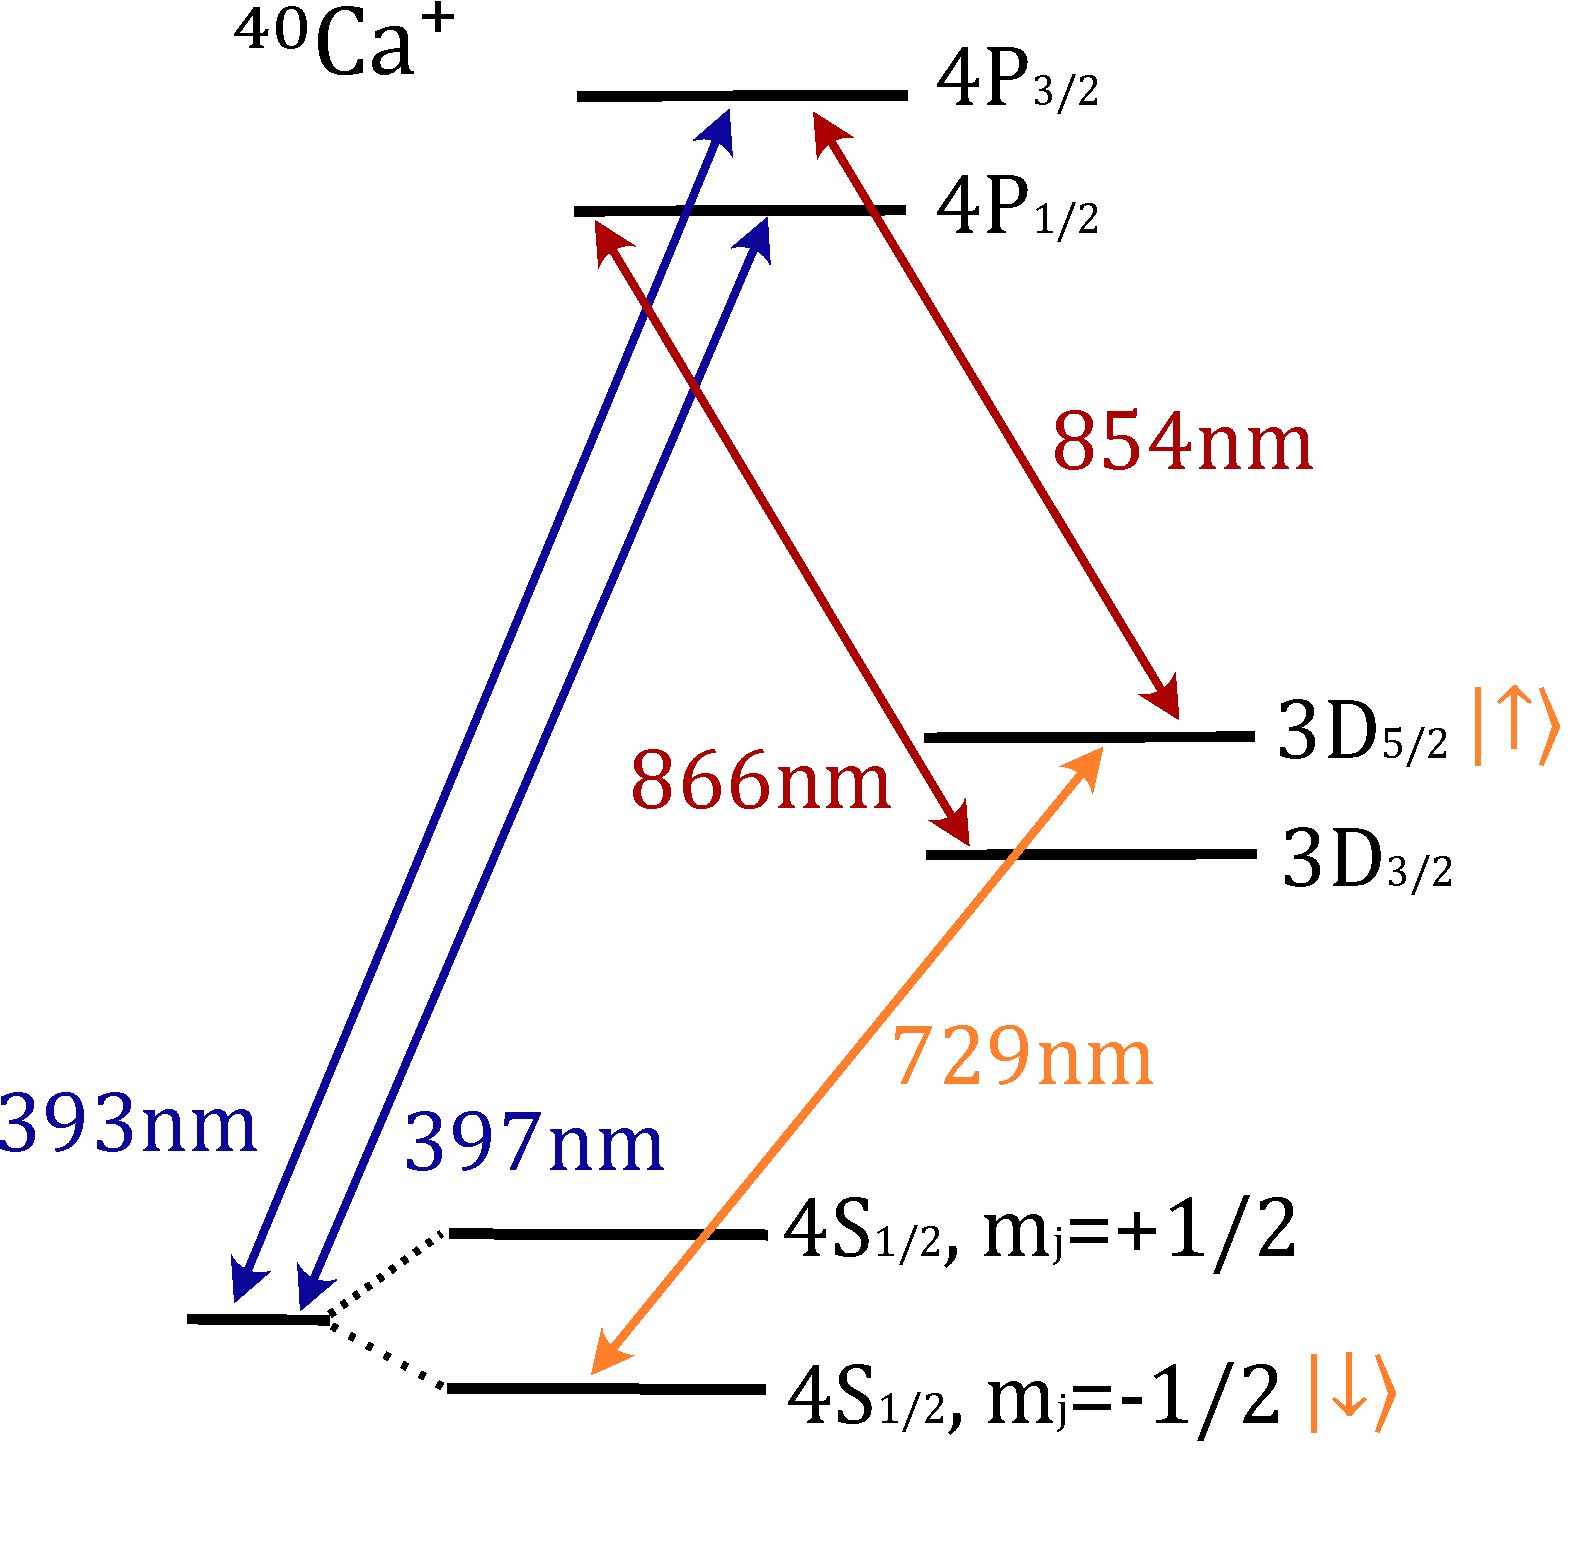
\includegraphics[width=0.4\linewidth]{figures/pdf_figure/Ca40.pdf}
        \end{center}
        \caption{
        Electronic energy levels of \textsuperscript{40}Ca\textsuperscript{+},
        which will be used in this thesis. The levels are
        split by the Zeeman effect due to a $5$~G external magnetic field (they are shown explicitely only for the ground state). The
        transitions marked are required for cooling and control over the
        ion. We shall use the optical-qubit with a quadrupole transition at
        729-nm. XXX TODO: Add zeeman levels for D5/2.
        }

    \label{fig:ion}
    \end{figure}

\section{The Ion Trap}
\label{sec:The Ion Trap}
% Main points:
    % Introduce the NPL trap chip and its advantages
    % Short intro into the parts of the ion trap DC/RF fields.
    % Fastino channels
    % Experimental parameters for stable trapping
    % Quote the values we use for trapping/experiment
% Pre reqs:
    % Motivation for trapping an ion!

    \begin{figure}
        \begin{center}
        \noindent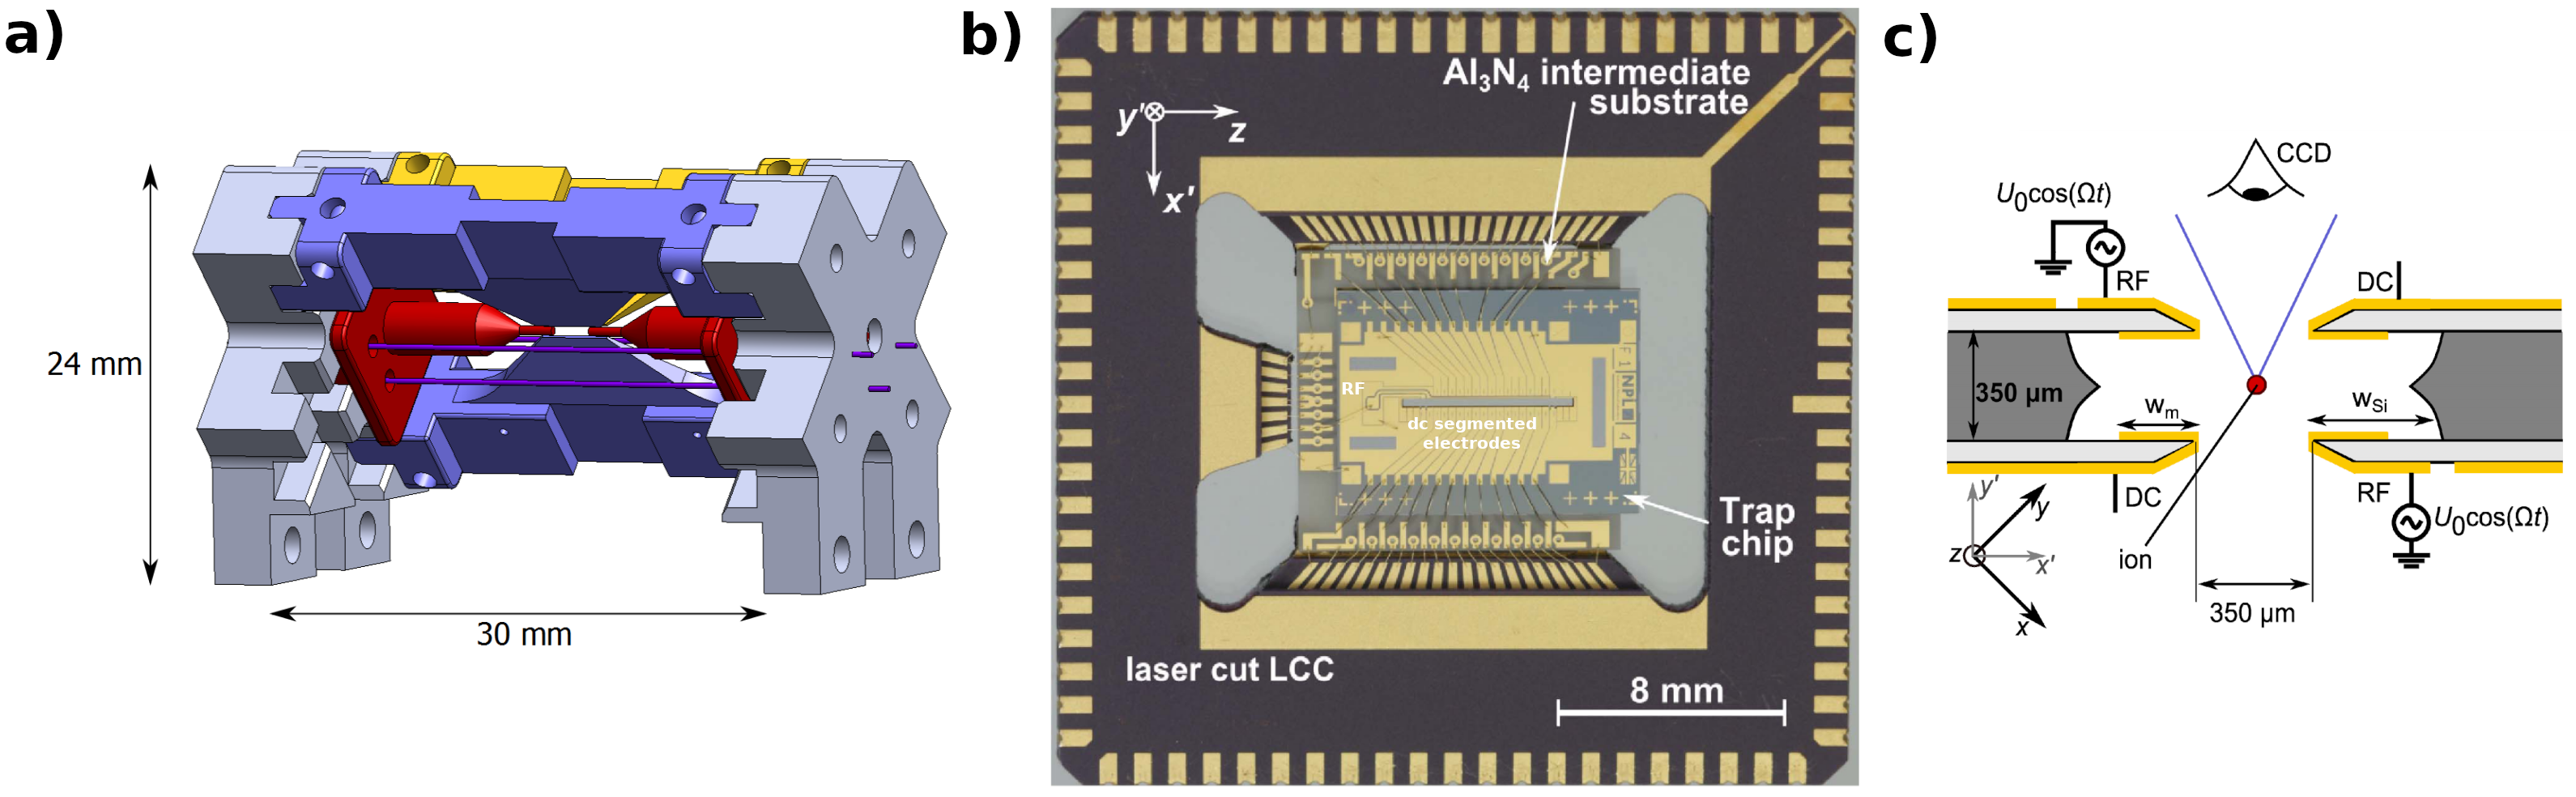
\includegraphics[width=\linewidth]{figures/png_figure/trap_comp.png}
        \end{center}
        \caption{\textbf{a)} XX Place holder figure. \textbf{b)} The NPL trap in use in this thesis. This is a microfabricated,
        segmented, multilayer trap. \textbf{c)} A cross sectional view of
        the NPL trap showing the RF and DC electrode positions.  Figures
        from~\cite{choonee_silicon_2017}.
        \label{fig:trap}}
    \end{figure}

    To create trapping potentials we use linear Paul traps, a schematic of such
    is shown in Figure~\ref{fig:trap}~(a). As explained by Earnshaw's theorem,
    $(\nabla^2 V = 0),$ a stable stationary point in 3D can not be realized
    using only static electric potentials, $V$, as if the potential is confining
    in two dimensions, it will be anticonfining in the third. Therefore, to
    achieve stable trapping either an oscillating electric field (Paul
    trap~\cite{XXX}), or a static magnetic field (Penning traps~\cite{XXX}) must
    be utilized to create a confining pseudopotential.\\
    Recently, the microfabricated surface style linear Paul trap has gained
    popularity due to the maturity of chip fabrication
    technologies~\cite{allcock_surface-electrode_2011} and the potential route
    to scalability this offers. In the surface trap, the 3D radial and axial
    electrodes of a ``macro'' trap are effectively projected onto a 2D surface.
    The stable point of such a trap is typically on the order of $50$ $\mu$m
    from the chip surface. The ease of fabrication of surface traps has allowed
    the creation of complex multizone devices with many DC electrodes.  These
    multizone traps enable the shuttling of ions, a requirement for Quantum CCD
    type architectures~\cite{kielpinski_architecture_2002}. However, this
    surface style geometry typically come with two costs: the depth of the
    trapping potential is often greatly reduced, and the close proximity of the
    surface to the ion can be a large contributor to motional heating
    rates~\cite{turchette_heating_2000}. \\
    The \emph{NPL} microfabricated 3D trap~\cite{see_fabrication_2013,
    wilpers_monolithic_2012}, as is used in our experiment, brings together the
    advantages of chip fabrication as well as the low heating rates and high
    trapping depths of a 3D style trap with greater ion-surface distances. This
    is achieved by a multilayer chip as shown in Figure~\ref{fig:trap}~(b, c).
    The radial trapping is provided by RF rails on opposite diagonals of the
    slit whilst axial trapping may be realized by the numerous DC electrodes.
    The ion-surface distance is now of the order $250$ $\mu$m and we have
    demonstrated heating rates of $ 33(3)$~q/s on a 4~MHz radial mode (see
    section~\ref{sec:Heating}).

    We aim for an axial ion separation of around $5$~$\mu$m which, for
    $^{40}$Ca$^{+}$ ions means a trapping potential of $\omega_z \approx 2\pi
    \cdot 1.6$~MHz. This ion separation was chosen to reduce the cross talk
    between ions when singly addressed (see section~\ref{sec:Single Addressing
    System}).\\ 
    We are targeting approximately $5$~MHz for our radial frequencies, as we
    shall use radial addressing for two-qubit entangling gates. The choice of
    this higher frequency is motivated by several factors. The Doppler cooling
    limit ($\overline{n} = \Gamma/\omega$, where $\Gamma$ is the transition
    linewidth and $\omega$ is the frequency of the cooled mode) inversely scales
    with the mode frequency. Consequently, higher mode frequencies result in
    lower temperatures following initial cooling. Additionally, a higher
    center-of-mass radial mode enables greater frequency separation of radial
    modes in a multi-ion crystal, which allow for greater selectivity of
    participating modes. \\ 
    Using the pseudopotential approximation~\cite{madsen_planar_2004} for the
    confining field, we can find a trapping frequency in one radial direction
    $\omega_p$
    \begin{equation}
    \omega_p = \frac{e\alpha V_{RF}}{\sqrt{2}\Omega_{RF}M\rho^2},
    \end{equation}
    where $\alpha$ is a factor of order unity given by the geometry of the trap,
    $V_{RF}$ and $\Omega_{RF}$ are the voltage and frequency provided to the
    RF-electrode, $M$ is the mass of the ion, and $\rho$ is the ion-RF electrode
    separation.  Applying some DC voltage on the axial electrodes leads to axial
    confinement with frequency $\omega_{ax}$, but must defocus the radial
    confinements as the total curvature of the pseudopotential must remain
    constant,
    \begin{equation}
    \omega_{rad} = \sqrt{\omega_p^2 - \omega_{ax}^2/2}.
    \end{equation}
    Due to the geometry of the DC electrodes with respect to the ion chain, the
    \emph{NPL} trap focuses one of the radial modes and defocuses the other when
    the DC electrodes are increased,
    \begin{equation}
    \omega_{rad\pm} = \sqrt{\omega_p^2 - (1\mp\beta)\omega_{ax}^2/2},
    \end{equation}
    where $\beta$ is some factor due to the geometry of this geometry. From
    simulation $\beta > 1$ for $\Omega_{RF} = 2\pi\cdot 23$~MHz and $V_{RF} =
    200$~V and so one radial mode increases with DC voltage applied and one
    decreases.

    \begin{table}[h!]
    \begin{center}
    \begin{tabular}{ c|c c c c c }
    & $V_{RF}$/V &  $V_{DC}$/V &$\Omega_{RF}$/($2\pi\cdot$MHz)& $\omega$/($2\pi\cdot$MHz)   & q \\ 
    &  &  & & $\omega_{ax}$\quad   $\omega_{rad}$ &  \\ 
    \hline
    Experiment  & 200 & -7 &  23 & 1.6 \quad 4.9 & 0.61 \\
    Loading  & 100 & -2 &  23 & 0.8 \quad 2.0 & 0.25 \\
    \end{tabular}
    \caption{ Simulated trapping parameters for both ``Experiment'' and ``Loading'' settings \textsuperscript{40}Ca\textsuperscript{+} with the NPL trap. The ``Experiment'' setting is optimized for high axial mode frequencies whilst the ``Loading'' setting maintains a lower q factor for practical loading.  \label{table:freqs}}
    \end{center}
    \end{table}

    A possible set of parameters to achieve $\omega_{ax} = 2\pi \cdot 1.6$~MHz
    and $\omega_{rad+} = 2\pi \cdot 4.9$~MHz can be seen in the ``Experiment''
    trapping in Table~\ref{table:freqs}.

    From the Mathieu equations, the areas of stability depend upon a factor
    $q$~\cite{berkeland_minimization_1998}, where
    $q=2\sqrt(2)\omega/\Omega_{RF}$.  Generally, we require $q$ to be as low
    ($q<0.3$) for convenient trapping.  To satisfy this requirement a
    ``Loading'' setting (with parameters in table~\ref{table:freqs}) may be used
    with $q = 0.25$ and then the $V_{RF}$ ramped to the ``Experiment'' trapping
    for high radial mode frequencies.

\subsection{Trap RF Chain}
% Main points:
    % Maybe a figure describing the elements within the RF chain
        % Frequency source (Urukul)
        % Resonator
        % RF rails
    % Quote values we use.
% Pre reqs:
    % NPL trap geometry

\subsection{Trap DC Voltages}
% Main points:
    % Describe Fastino DAC and the available electrodes on the NPL trap
    % Quote values we use.
% Pre reqs:
    % NPL trap geometry

\section{Beam Geometries and Vacuum System}
\label{sec:Vacuum System}
% Main points:
    % Technical drawing of beam geometries and magnetic field to ion chain.
    % Drawing of ion trap package with high NA lenses
    % Standing waves at the ion
% Pre reqs:
    % NPL trap
    % Why we have Dual high NA lenses
    % Magnetic field giving Zeeman shift

\begin{figure}
  \begin{center}
   \noindent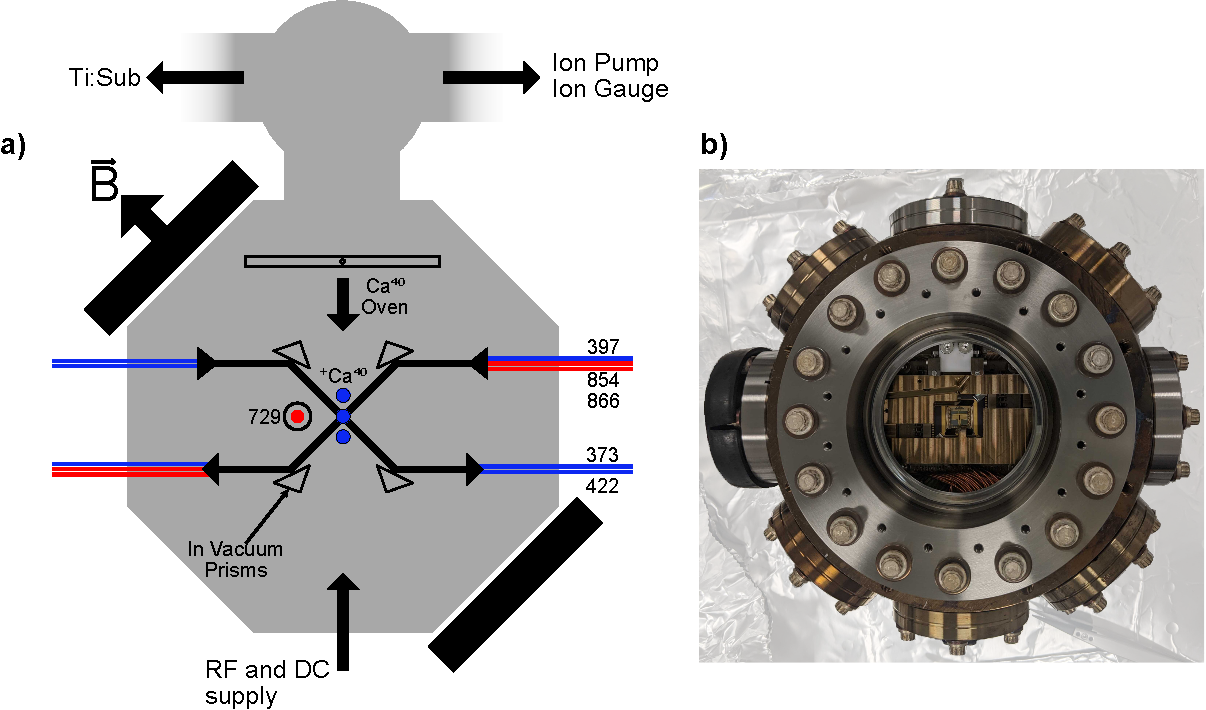
\includegraphics[width=0.9\linewidth]{figures/pdf_figure/vacuum_can-crop.pdf}
  \end{center}
  \caption{
    \textbf{a)} XXX Place holder figure. A schematic of the vacuum chamber.
    Wavelengths apart from 729-nm enter through the side CF40 viewports and are
    directed onto the ions by in vacuum prisms. The 729-nm light enters through
    the larger CF100 viewports.  \textbf{b)} A photograph of the assembled
    system prior to baking.
  }
  \label{fig:can}
\end{figure}

\subsection{Vacuum System}
% Main points:
    % List of used parts
    % What is inside the system and what is its contruction/materials
    % Operation of ion pump/Ti:Sub
% Pre reqs:

\subsection{Optical Access}
% Main points:
    % Dual High NA repeat?
    % NA for readout
    % NA for single addressing?
    % In vacuum prisms spec and design
% Pre reqs:
    % Trap package
    % Vacuum system

\begin{figure}
  \begin{center}
   \noindent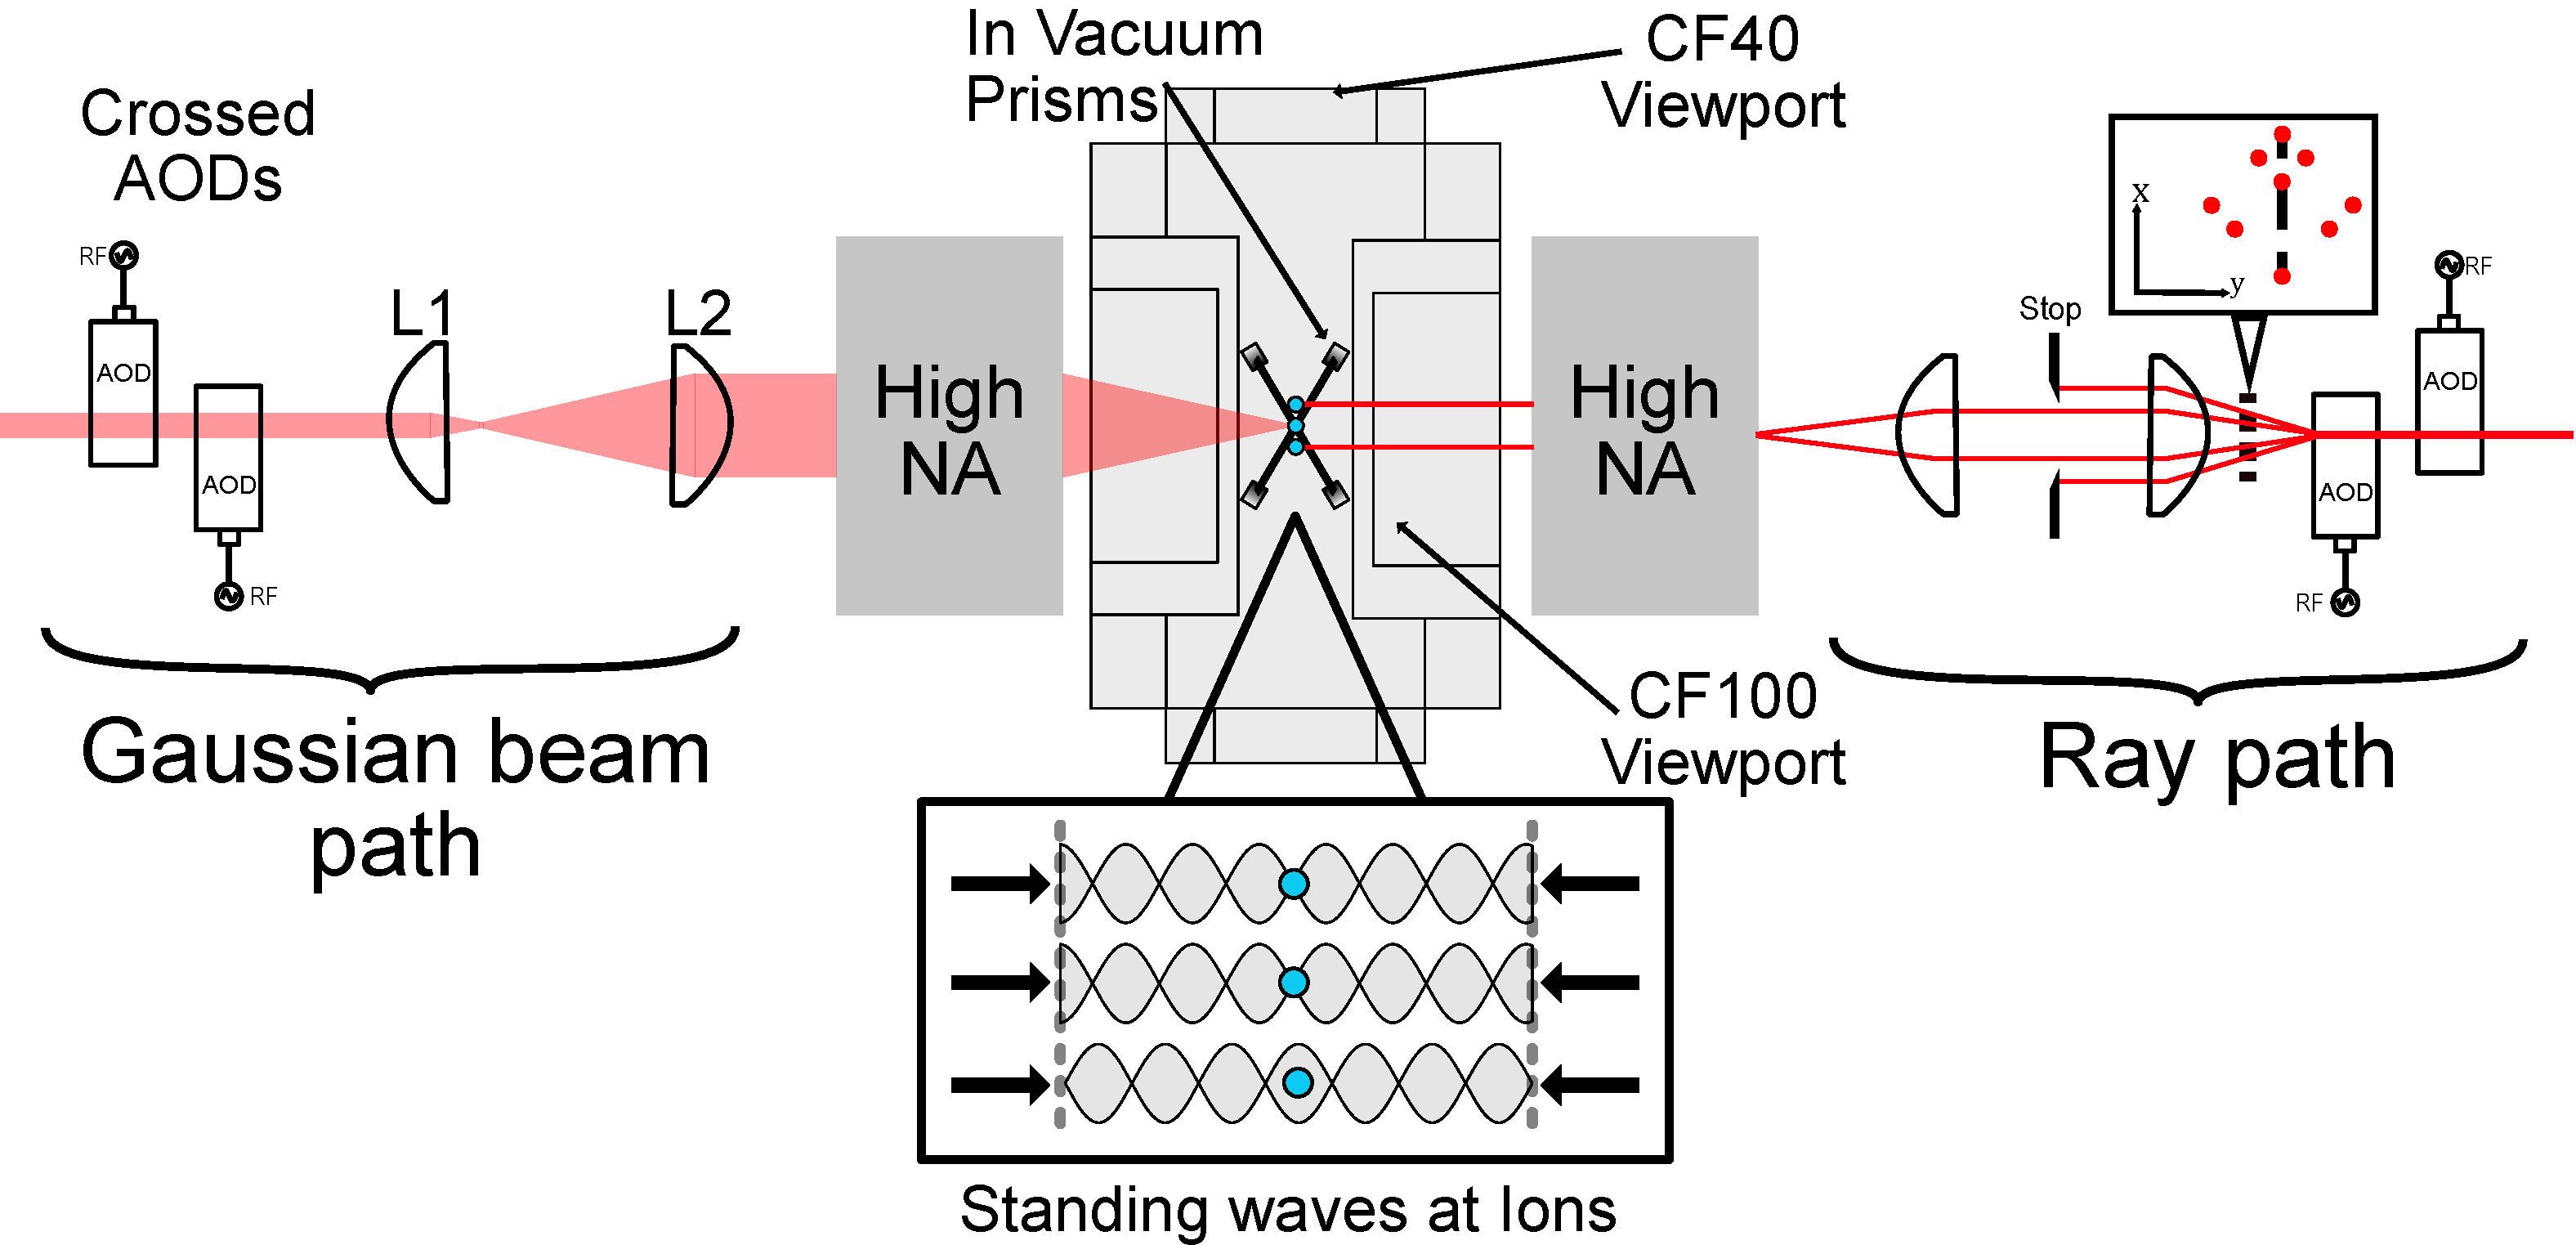
\includegraphics[width=\linewidth]{figures/pdf_figure/vac_can_AOD_small.pdf}
  \end{center}
  \caption{XXX Place holder figure. The standing wave single addressing system. Dual high NA
    objectives focus the light to a tight waist at the ions
    location. AODs are used to steer the light to only selected
    ions. The left hand side of the figure shows the Gaussian profile
    of the light, whilst the right hand side shows a ray
    representation of how two singly addressing spots are formed at
    the ions. L1 is a telecentric scanning lens and in combination
    with L2 form a beam expander.}
  \label{fig:AOD}
\end{figure}

\section{Ca$^+$ Laser Systems}	
\label{sec:Laser systems}
% Main points:
    % State which lasers we need access to
    % What frequency control do we need on each? PDH lock, AOM etc.
    % Table of all AOMs and offset frequencies
    % Table of laser powers in mW and with aimed saturation intensities for doppler idle, cooling, readout, and laser linewidths.
% Pre reqs:
    % Calcium level structure
    % 5 G field

\subsection{Narrow Line Width 729 Laser}
\label{sec:Narrow Line Width 729 Laser} 
% Main points:
    % What equipment does the 729 consist of.
    % Solstis cavity
    % Beam path and control loops (PDH, FNC)
    % Frequency shifting, pulse carving via urukul
    % Amplitude stabilisation with SUServo
% Pre reqs:
    % Calcium level structure

    Lasers are a key tool for creating the highly localised, strong electric
    field amplitudes and gradients needed to drive both carrier and sideband
    transitions of the trapped ion.\\ As shown in Figure~\ref{fig:ion}, we will
    use two levels within the 4S\textsubscript{1/2} to 3D\textsubscript{5/2}
    manifolds to define our qubit. This is an electric quadrupole transition as
    $\Delta l = 2$.  For the Calcium ion this transition is at 729-nm, and so we
    use a near resonance 729-nm laser to implement single- and multi-qubit gates
    (sections~\ref{sec:Randomised Benchmarking} and~\ref{sec:Two-Qubit
    Entangling Gates}). We also use this transition, after Doppler cooling, for
    resolved sideband cooling to bring the motional mode close to its ground
    state (as discussed in section~\ref{sec:Cooling}).

    This transition is narrrow line width due the the long lived
    3D\textsubscript{5/2} state, and so, for power efficiency, we must use a
    narrow linewidth laser. For our ``fast entangling gates'' use case we
    require large electric-field intensities at the ion to drive sideband
    transitions, this will be discussed further in the single-addressing and
    two-qubit gate sections, but here it is sufficient to say we require >100 mW
    of light at the ion plane.  Here we describe the built system 
    consisting of a Ti:Saph laser system pumped with by an Nd:YAG 532-nm laser.\\

    We pump an \emph{M2 Solstis} Ti:Saph~\cite{XXX} with 18 W of 532-nm light
    from a \emph{Coherent Verdi-V} system~\cite{XXX} to produce around 5W of
    729-nm light.  The Ti:Saph is engineered to operate with a stable $<50$~kHz
    linewidth. Ti:Saph crystals have broadband gain profiles~\cite{XXX}, which
    is often exploited in research environments to create frequency tunable
    laser systems. We however want a narrow linewidth, single frequency laser,
    and so the \emph{Solstis} has multiple intracavity frequency selective
    elements. These consist of (in order of coarse frequency selectivity), a
    birefringent filter, a tunable Fabry-P\'erot etalon, and the surrounding
    bow-tie cavity. For stable single mode operation, the \emph{Solstis} employs
    an active ``dither" servo to lock the peak of etalon transmission to one of
    the cavity longitudinal mode. This dither consists of periodically varying
    the etalon spacing with a frequency of around 20~kHz. We must be aware of
    this dither frequency as the phase modulation leads to the creation of
    sidebands on our light which can interact with the ion causing unexpected
    errors in gates. We can observe this dither frequency (and harmonics of it)
    with our ion via composite pulse experiments, however it is currently not
    expected to be a limiting source of error in any of our desired interactions
    we study.\\
    \begin{figure}
    \begin{center}
    \noindent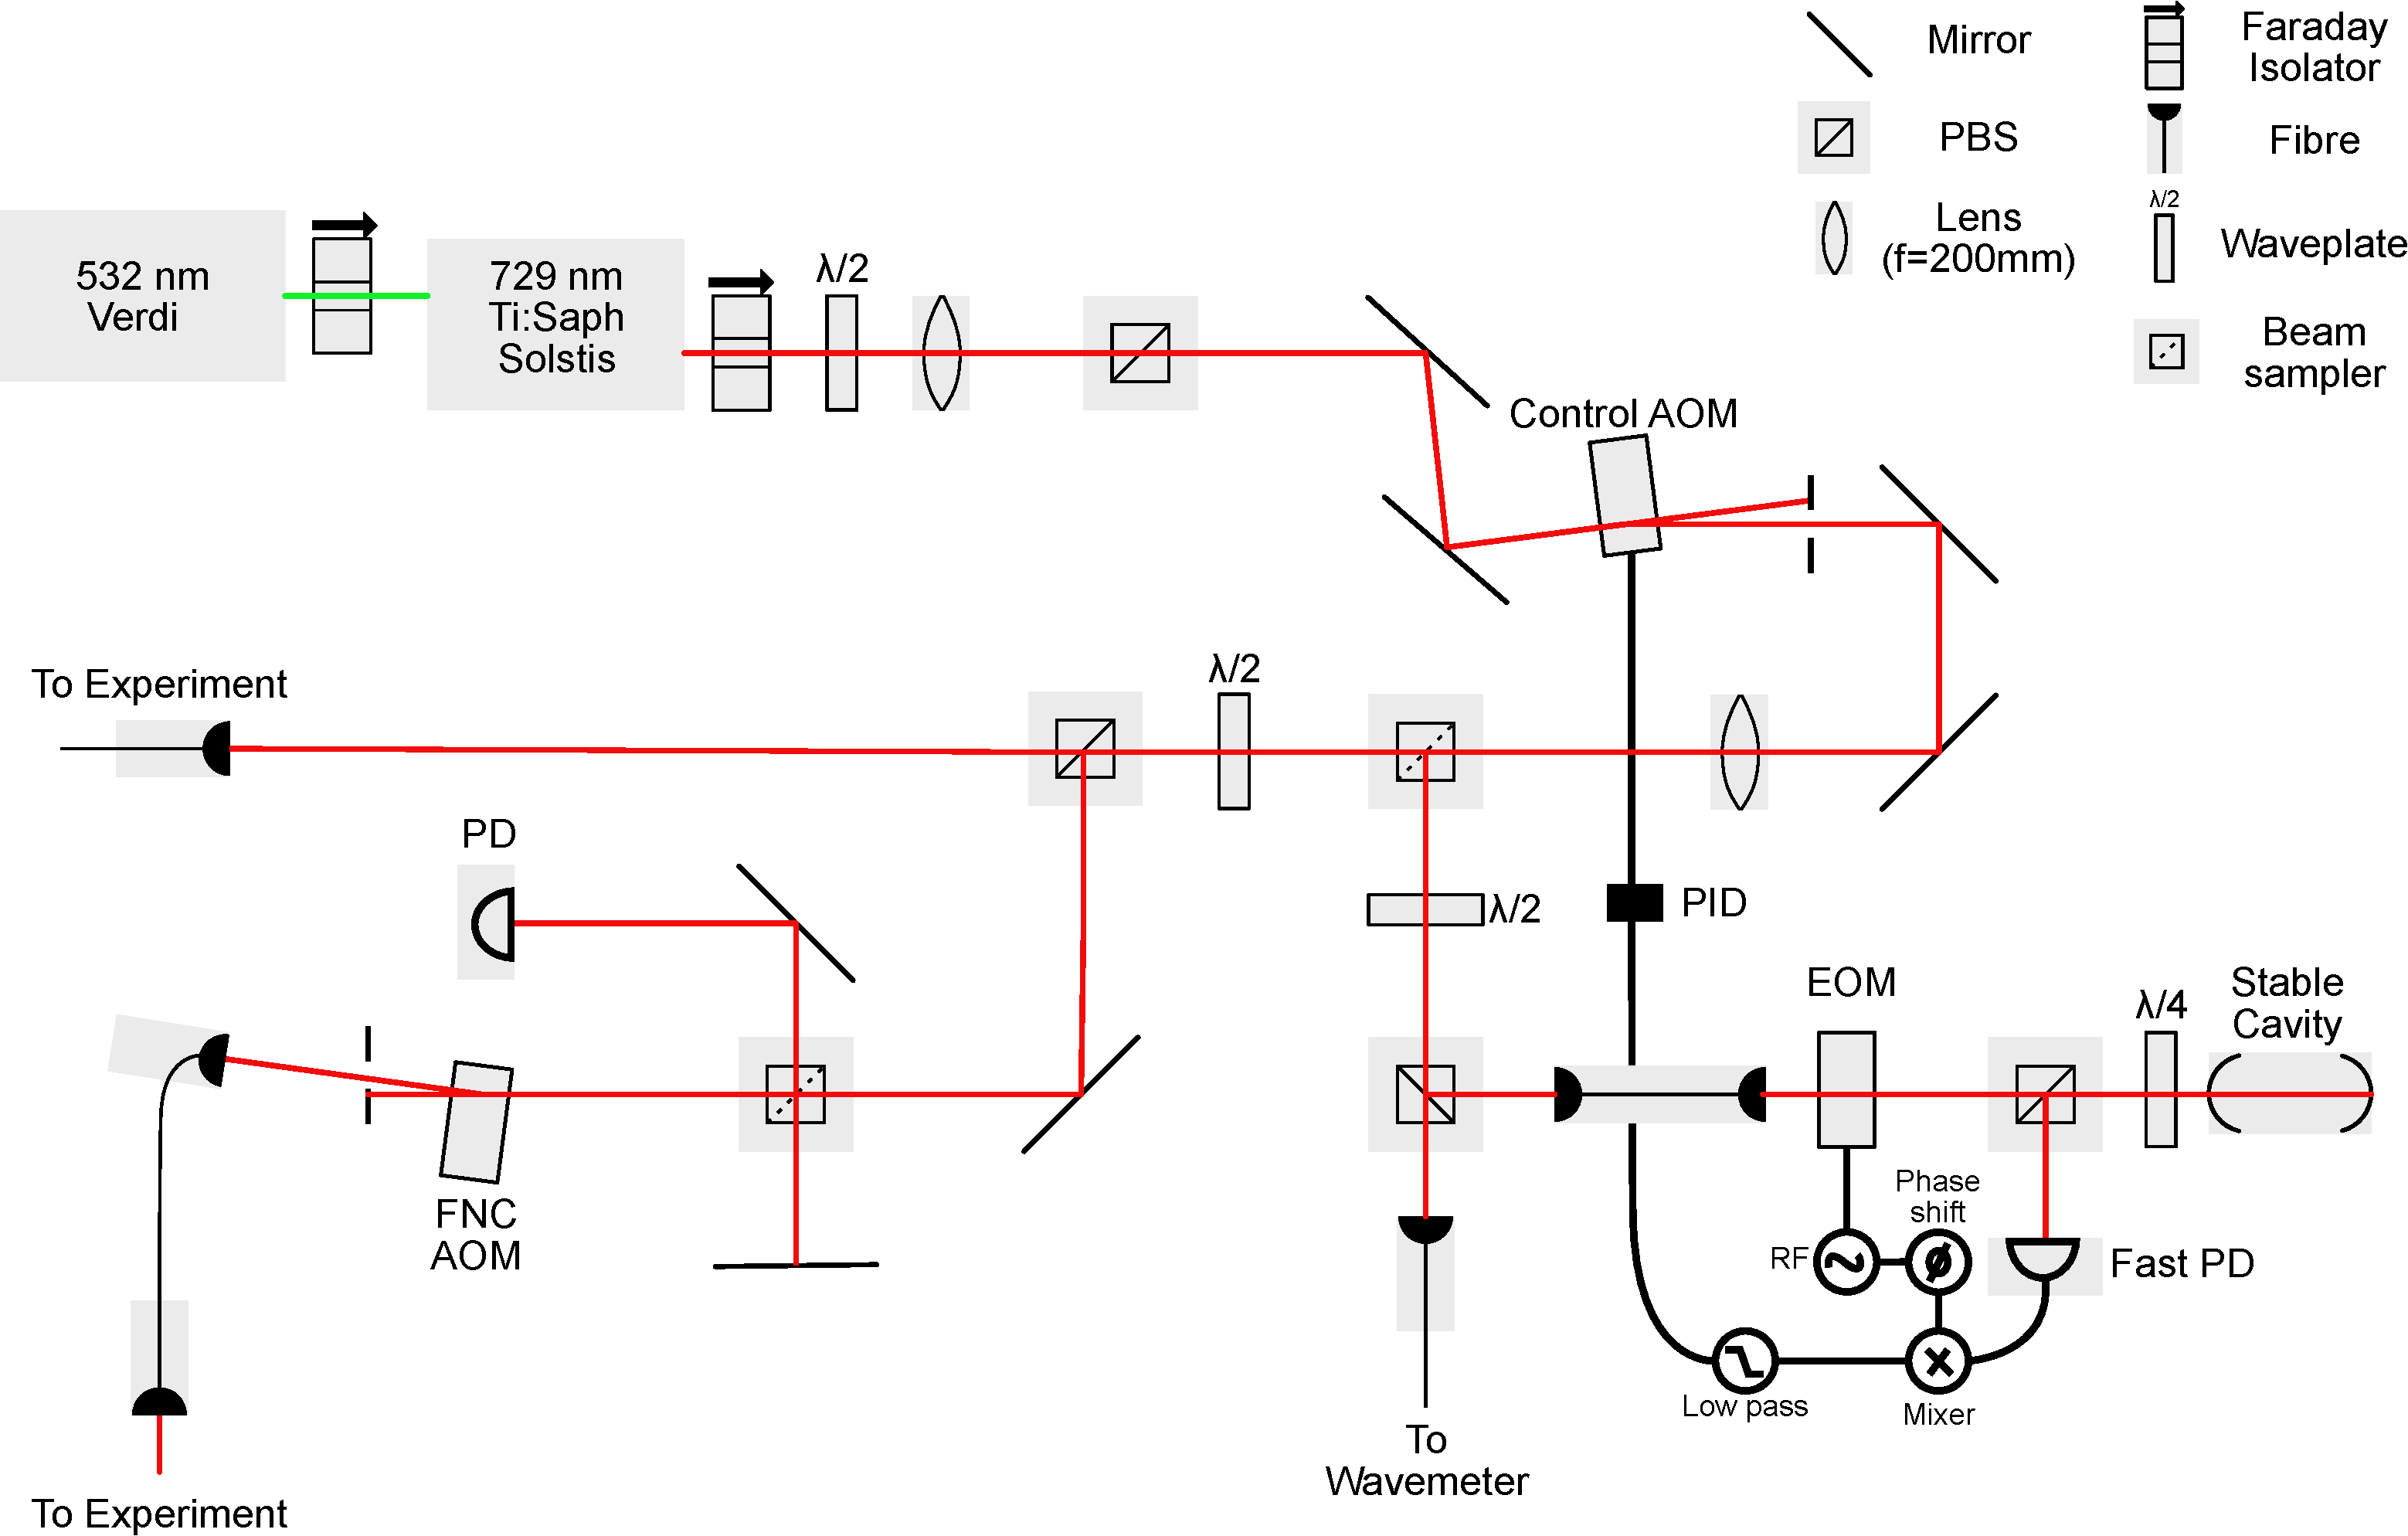
\includegraphics[width=0.9\linewidth]{figures/pdf_figure/729_path_small.pdf}
    \end{center}
    \caption{The 729-nm system. A Ti:Saph laser tuned to 729-nm is
        pumped by a 532-nm source. Light is picked off at the first beam
        sampler to stabilise by PDH locking to a cavity.}
    \label{fig:729}
    \end{figure}
    \begin{figure}
        \begin{center}
        \noindent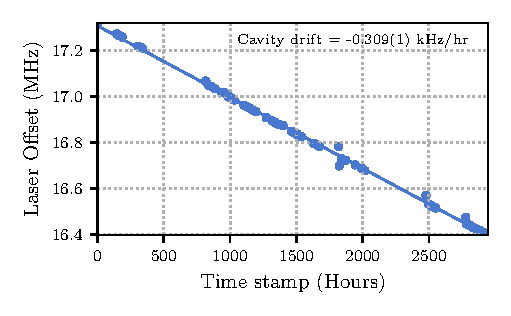
\includegraphics[width=\linewidth]{
            figures/pdf_figure/cavity_drift.pdf
            }
        \end{center}
        \caption{
            Cavity drift over 125 days. Extracted by reference to ion transition.
            }
        \label{fig:Cavity Drift}
    \end{figure}
    As mentioned, the \emph{Solstis} alone can operate with linewidths of
    $<50kHz$, however we push this further by referencing the Ti:Saph output
    with an ulta high finesse cavity by \emph{Stable Laser Systems} and applying
    a Pound-Drever-Hall (PDH) lock~\cite{}.  A schematic of our 729-nm system is
    shown in Figure~\ref{fig:729}.  PDH locking requires applying two sidebands
    via an electro-optical modulator (EOM) to the light and directing it onto
    the stable cavity. The light reflected from the cavity is then directed onto
    a fast photodetector (\emph{Thorlabs PDA10A2}). The reflection from the
    cavity consists of the interference between the carrier and the sidebands
    which have been respectively altered by the cavity transfer function. The
    photodetector signal is mixed down with the same oscillator signal as
    provided to the EOM but delayed by some chosen phase, and finally low pass
    filtered to produce a signal for use as the error signal in the servo loop.
    This error gives a measure for how far the carrier frequency is from the
    stable cavity resonant frequency and is used for feedback onto the control
    AOM situated after the Solstis. The electronics for this control loop are
    provided also by Stable Laser Systems in the form of their \emph{FPGA Servo}
    lock box. For an effective PDH lock, we require both short and long term
    stability of our reference cavity. To ensure the cavity is insensitive to
    the environment, it is made of an ultra low expansion material. We
    temperature stabilise the cavity at the zero crossing temperature of
    $30.6^\circ$C, and it is further isolated by being stored in a vacuum system
    at $<1e-7$~mbar. We measure a long term cavity drift of 309(1) Hz/hr over
    125 days, seen in figure~\ref{fig:729}. This measurement uses the ion as a
    frequency reference to probe the cavity frequency and is discussed in
    section~\ref{sec:Laser Offset}.\\
    Figure~\ref{fig:729} displays the other beam paths for our 729-nm system.
    Some light is picked off and sent to a wavemeter to continuosly monitor the
    frequency. However, the majority is coupled to two output fibres for our
    experiment and another within the group. We transport the 729-nm light from
    a dedicated laser lab to a room containing the trap apparatus by a 10~m
    single mode polarization maintaining fibre (\emph{SKXXX}).  The fibre is
    beneficial in cleaning up the mode from the Ti:Saph, however it can
    introduce phase noise due to mechanical and thermal effects along the 10~m
    length. To remove this introduced noise we utilise passive stabilisation in
    the form of thick foam tubing along the fibre length as well as active
    stabilisation by popular fibre-noise-cancellation technique~\cite{XXX}. This
    topic has been discussed extensively in multiple PhD and Masters
    theses~\cite{XXX}, and so here we only quote the relevant control aspects of
    our arrangement. We use the \emph{Sinara Stabilizer}~\cite{XXX} board, a
    dual channel PID microcontroller, with the \emph{Pounder}~\cite{XXX}
    mezzanine board, a dual channel PDH lock generator. The FNC PID software was
    developed by Ayush Agrawal ~\cite{XXX}. A comparison of spin coherence times
    is shown in section~\ref{sec:Coherence} with and without fibre noise
    cancellation enabled. \\


\subsection{Single Addressing System}
\label{sec:Single Addressing System}
% This section is not used in any characterisation - could be left for outlook!
% Main points:
    % The advantages of single addressing using AODs
        % Ion selectivity
        % High intensity electric field
    % single addressing system creating standing waves
    % render of single addressing system
% Pre reqs:
    % 729 system
    % High NA
    % Trap package
    % Motivation for future experiments

% ------------------------------------------------------------------------

\chapter{Experiment Characterisation}

    Before we can dive into running novel experiments involving the motion and spin
    of the atoms, we need to characterise our apparatus. This allows us to both
    benchmark our system against state of the art results, and to reveal any
    current limitations of the apparatus which we may need to address.

\section{Quadrupole Transitions}
\label{sec:Transitions}
% Main points:
    % All visible motional modes on large detuning scan at $5$~G. 
    % Can compare when have all quadrupole transitions available or when we selectively omit transitions via polarisation.
% Pre reqs:
    % 5 G field

\section{Spin}
\label{sec:Spin}

\subsection{Rabi and Ramsey Scans}
% Main points:
    % The ion is a sensor!
    % Method for Rabi and Ramsey scans
    % Mention changing polarisation to select certain transitions
    % Long Rabi flop
    % Likely reason for flop damping
    % Measuring detuning using Ramsey scan
% Pre reqs:
    % 729 system
    % Available Quadrupole transitions

    \begin{figure}
        \begin{center}
        \noindent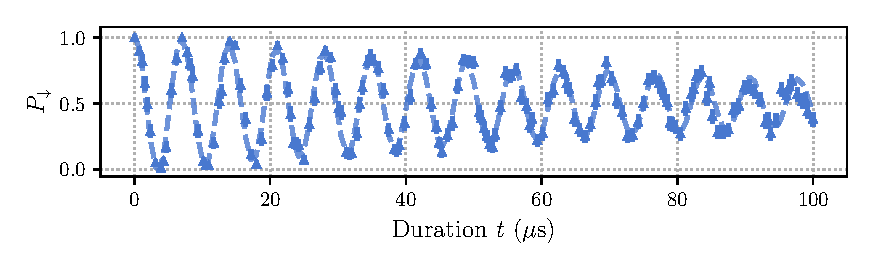
\includegraphics[width=\linewidth]{
            figures/pdf_figure/long_flop.pdf
            }
        \end{center}
        \caption{Long duration Rabi Flop with fitted decaying flop.
            }
        \label{fig:Long Flop}
    \end{figure}

    Here we briefly describe the method in which we extract Rabi frequencies and single qubit gate durations.
    Long Rabi flop (100 us), fit out carrier frequency of 2*pi*0.0716(1) MHz and
    Decay rate of $0.0107(7)$ 1 / us. See long flop. This is 1 mW of power on m1\_m3
    transition before we changed polarization. Fit with decaying cos function 
    \begin{equation}
        \frac{1 + e^{-\lambda t} \cos(2 \Omega t)}{2},
    \end{equation}
    % 1 mW 729~nm laser -> Fit out pi/2, pi, 2pi pulses. We are using square pulses.


\subsection{Spin Coherence Times}
\label{sec:Coherence}
% Main points:
    % Quote coherence times comparing:
        % Mumetal box panels
        % Transitions with diff mag sensitivity
        % FNC/ no-FNC
% Pre reqs:
    % MuMetal box
    % Available transitions
    % 729 laser system

    Individual gate fidelities are ultimately limited by loss of coherences of
    the two qubit states due to either dephasing or by the natural lifetime of the upper level. By our choice of ion and qubit levels, defined between
    the ground $4S_{1/2}$ state and the metastable $3D_{5/2}$ state, we can
    expect a lifetime limited coherence time of $\tau = 1.1$~s~\cite{}. 
    %Barton, P. A. et al. Measurement of the lifetime of the 3d 2D5/2 state in
    %40Ca+.Physical Review A 62, 032503 (2000).
    In practise, mainly due to imperfect tracking of laser frequency and
    magnetic field drifts (as mentioned above), we see coherence times dominated
    by dephasing. To discern between these two noise sources, we may exploit the
    fact that we have multiple Zeeman levels within our $3D_{5/2}$ state with
    varying magnetic field sensitivities. We also have the ability to define our
    qubit on the Zeeman split ground state, which decouples dephasing due to the
    laser from measured coherence times. We perform Ramsey scans with varying
    mid-sequence delay durations to extract the coherence times, an example of
    which can be seen in figure~\ref{fig:coherence_times}. In characterising the
    spin coherence times, we hope to explore both the efficacy of the magnetic
    shielding surrounding the ion trap, as well as the stability of the 729~nm
    laser. \\
    Figure~\ref{fig:coherence_times} shows how the magnetic shielding effect
    coherence times of three transitions, XX, YY and ZZ, with magnetic field
    sensitivities of XX, YY and ZZ respectively.  From this we find that without
    the shielding, we are strongly limited by external magnetic field noise, and
    with full sheilding we suppress this noise to where we are dominated by
    laser phase noise. To find the factor by which the magnetic field noise is
    attenuated, we can compare the coherence times of the laser phase
    insensitive transition with and without the box. We find an attenuation
    factor of XX, which is XXconsisitent with the expected attenuation factor of
    the mu-metal shielding.\\
    With the shiedling in place, we compare the coherence times of the
    $4S_{1/2}, m_j = -1/2 \leftrightarrow 3D_{5/2}, m_j = -5/2$ with fibre noise cancellation (see
    section~\ref{sec:Narrow Line Width 729 Laser}) and without, figure~\ref{fig:coherence_times}. We find that the
    coherence time is improved by a factor of XX, with FNC enabled. Our current
    spin coherence time of XX~ms is limited by the laser phase noise, and we
    expect to be able to push this to [ref R. Oswald] by improving the laser PDH
    stability. However, for the immediate planned experiments (see
    section~\ref{Outlook}), these improvements will be a low priority due to
    other likely dominating error sources in the motion of our ions.\\

\subsection{State Preparation and Measurement}
% Main points:
    % Method of preparation via optical pumping
    % Readout characterisation with NA 0.6 lens
    % Compare readout histograms of fast 30 us readout to Doppler cold 100 us readout
    % Quote state prep error (back this from RBM + measurement histograms)
% Pre reqs:
    % Laser systems powers
    % 729 system
    % Available transitions
    % pi-pulses

    To utilise two levels of the ion as a qubit, we need to be able to
    selectively prepare the ion into one of the Zeeman levels of the ground
    state. As mentioned in section~\ref{sec:Magnetic Field}, we are operating at
    a low magnetic field of 5~G, leading to a splitting between the Zeeman
    levels of less than 21~MHz, the natural linewidth of the 397~nm transition.
    This means we cannot optically pump using 397~nm frequency selectivity.
    Further, due to the constraint of beam geometry from the in vacuum optics,
    we can not use polarisation selectivity of the 397~nm transition. Instead,
    we use the narrow line width 729~nm laser on resonance with the $4S_{1/2},
    m_j = +1/2 \leftrightarrow 3D_{5/2}, m_j = -3/2$ transition, and the 854~nm
    deshelving laser on resonance, to optically pump into the $m_j = -1/2$
    Zeeman level we define as our qubit ground state. \\
    To measure the qubit state of the ion, we apply the 397~nm and 866~nm lasers
    and count 397~nm photons scattered. From the level diagram shown in
    figure~\ref{fig:level_diagram}, we can see that upon turning on the 397~nm
    laser, if we are in $|0\rangle$, photons will be scattered, and if we are in
    $|1\rangle$, then no photons will be scattered. To optimise the fidelity of
    measurement we ensure that the signal is discernible with low error from any
    background counts on the camera. In general, improving the number of signal
    counts can be achieved by tuning the 397~nm laser near to the transition
    resonance, by increasing the readout duration, or by increasing the
    percentage of scattered photons captured by the imaging system. Practically
    we desire that the readout step does not heat the motion of the ion and so
    we red detune the 397~nm laser to a similar setting as for Doppler cooling
    (see section~\ref{sec:Cooling}). The parameters we use for readout are
    summarised in table~\ref{tab:readout_parameters}, and a typical histogram of
    readout counts for one and two ions can be seen in
    figure~\ref{fig:readout_histogram}. We find that the readout fidelity is
    XXX.\\
    To measure the effect of state preparation and measurement error on longer
    experimental sequences, we will discuss randomised benchmarking in the following
    section~\ref{sec:Randomised Benchmarking}. Due to the relevance here, we
    quote the measured state-preparation and measurement error (SPAM) of $\epsilon_{SPAM} = 1.46(6) \times 10^{-3}$.\\
    
\subsection{Randomised Benchmarking}
\label{sec:Randomised Benchmarking}
% Main points:
    % Here is a characterisation of single qubit gates.
    % Explain RBM method
    % Quote values measured
    % What is likely error source
    % Are we limited by this error?
    % What is state of the art (for optical quadrupole transition)
    % What contribution is the spin coherence time?
% Pre reqs:
    % Spin coherence times
    % Possible transitions
    % Calibrating gate times

    \begin{figure}
        \begin{center}
        \noindent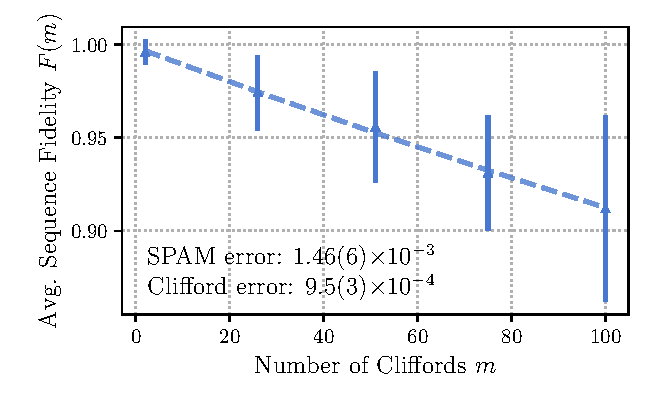
\includegraphics[width=\linewidth]{
            figures/pdf_figure/rbm_fit.pdf
            }
        \end{center}
        \caption{
            RBM fit
            }
        \label{fig:rbm}
    \end{figure}

    High fidelity unitary operations (gates) are essential for both near
    intermediate scale quantum computing and for reducing overheads in required
    physical qubits and operations in fault-tolerant
    schemes~\cite{steane_overhead_2003}. To evaluate the quality of both our
    state-prep and single qubit rotations, we employ randomized benchmarking
    (RBM)~\cite{knill_randomized_2008, magesan_scalable_2011}.  RBM consists of
    applying random combinations of a pre-chosen discrete set of gates to
    estimate an average error per gate.  We chose the single-qubit Clifford
    group as our set of gates to evaluate. The single-qubit Clifford group is
    the set of unitaries which map the Pauli matrices to one another through
    conjugation. This can be thought of as the complete set of rotations of the
    Bloch sphere such that all valid combinations of the axis $(x \rightarrow
    \{\pm x,~\pm y,~\pm z\}),~(y \rightarrow \{\pm x,~\pm y,~\pm z\}),~(z
    \rightarrow \{\pm x,~\pm y,~\pm z\})$ are realized. There are 24 unitaries
    in this set. We followed the RBM protocol described in the
    Thesis~\cite{hughes_benchmarking_2021} to evaluate our single-qubit gates.
    First the qubit is prepared in some known initial state, i.e. prepared in
    some chosen basis. A gate sequence is then applied which consists of
    multiple random Clifford gates followed by a final `inverting' Clifford,
    where the `inverting' Clifford is chosen such that the full sequence
    performs the Identity operation. The state is then measured in the same
    basis to find any deviations from the Identity being performed due to gate
    errors. This is repeated with the same preparation and sequence multiple
    times to calculate the probability that the Identity was performed - thus
    giving the sequence fidelity. These steps are repeated for many different
    random sequences with a range of sequence lengths. The decay model we fit to
    the fidelity versus number of Clifford gates is given by,

    \begin{equation}
        F(m) = \frac{1}{2}\left( 1+(1-2\epsilon_{SPAM})(1-2\epsilon_c)^m\right),
    \end{equation}

    \noindent where $F(m)$ is the fidelity of the sequence of length $m$,
    $\epsilon_{SPAM}$ is the state-preparation and measurement error, and
    $\epsilon_c$ is the average error per Clifford gate.  We use this method to
    bench mark our qubit transition. The Clifford gates are decomposed into
    sequences of $\pi/2$ and $\pi$ pulses about either the $x-$ or $y-$axes. We probe up to $m=100$ Clifford gates, and fit the decay of the fidelity to the above model.
    We measure the error per Clifford to be $\epsilon_c = 9.5(3) \times 10^{-4}$,
    while the SPAM error is $\epsilon_{SPAM} = 1.46(6) \times 10^{-3}$. The decay plot for
    this RBM sequence can be seen in figure~\ref{fig:RBM_decay}. The error bars
    are given by the standard deviation of the survival populations. There are on average 3.50 $\pi/2$ pulses per Clifford, with a typical $\pi/2$ duration of $1.3~\mu$s.\\


\section{Motion}
\label{sec:Motion}
% Main points:
    % Quote characterisation method and values for various motional measurements.
    % Highlight where we are not yet at the capability we need.
    % State what improvements we plan to add.
% Pre reqs:
    % Motivation for control of motion of ion
    % Trap RF DC
    % Laser systems

\subsection{Cooling}
\label{sec:Cooling}
% Main points:
    % Introduce why we want to cool
    % Doppler cooling
    % Sideband cooling
% Pre reqs:
    % Motional mode and beam geometry
    % Laser systems 
    % Trapping

    For any interaction involving the motion of the ion, we require both the
    ability to prepare the motional state with high fidelity, and to
    subsequently measure this motional state to verify correct preparation. For
    entangling gates, and the creation of squeezed states which we are
    considering in this chapter, we assume that we begin in the motional ground
    state, or in other words, Fock state zero.  Our initially trapped ions will
    be in some high temperature thermal state, (*given by the oven temperature
    and the PI laser momenta kicks*). We first doppler cool our ions, and then
    subsequently sideband cool them. We give a brief description of these two
    cooling processes here.\\

\subsubsection{Doppler Cooling}
% Main points:
    % Quote final temperature reached (theory?)
    % Describe cooling parameters
% Pre reqs:
    % Motional mode and beam geometry
    % Laser systems 

    Doppler cooling exploits the fact that incident light onto a moving ion will
    appear frequency shifted in the rest frame of the ion. For Doppler cooling
    of $^{40}$Ca$^+$, we apply both the 397~nm and 866~nm lasers. We initially red
    detune the 397~nm laser by around 100~MHz. This results in the preferential
    absorption of a quanta of 397~nm light by ions with a velocity vector
    antiparallel photon k-vector. After this absorption, the ion will be in the
    excited $4P_{3/2}$ state and spontaneously decay to either the $4S_{1/2}$,
    or the $3D_{3/2}$ emitting a photon of either 397~nm or of 866~nm
    respectively into a random direction. These two decay paths have a branching
    ratio of XX.  As we desire many photon kicks to cool our ions, we repump the
    electron out of this metastable $3D_{3/2}$ level by applying an on resonant
    866~nm beam.  The absorption and sequential emission of this 397~nm photon
    will lead to a net reduction in the motional energy of the ion if the photon
    is emitted at a higher energy than when absorbed. The equilibrium
    temperature is given by the condition where the doppler cooling rate is
    equal to photon recoil heating of the ion. Assuming a Lorentzian absorption
    profile, the minimum temperature is given by,
    \begin{equation}
    T_{Doppler} \approx \frac{\hbar\gamma}{2k_B},
    \end{equation}
    where $\hbar$ is the reduced Planck constant, $\gamma$ is the natural
    linewidth of the transition, and $k_B$ is Boltzmann's constant.\\ For
    $^{40}$Ca$^+$, the natural linewidth of the 397~nm transition is $\frac{\gamma}{2\pi} =
    21$~MHz, leading to a Doppler temperature of approximately 0.5~mK. Given a radial mode frequency of $\frac{\omega}{2\pi} = 4$~MHz, and the mean occupation number of the oscillator being given by,
    %[ref NIST https://www.physics.nist.gov/PhysRefData/Handbook/Tables/calciumtable4.htm] 
    \begin{equation}
        \bar{n} = \frac{1}{e^{\hbar\omega/k_B T}-1},
    \end{equation}
    we find the final thermal distribution to have an expected Fock state of $\bar{n} = 2.3$.
    Using parameters summarised in table~\ref{tab:cooling_parameters}, we find practically the final temperature after Doppler cooling to be around XXX~mK.\\

\subsubsection{Sideband Cooling}
% Main points:
    % Quote final temperature reached
    % Describe SBC pulse sequence
    % We use a closed transition
% Pre reqs:
    % Motional mode spectra
    % Laser systems 
    % Rabi flopping

    \begin{figure}
        \begin{center}
        \noindent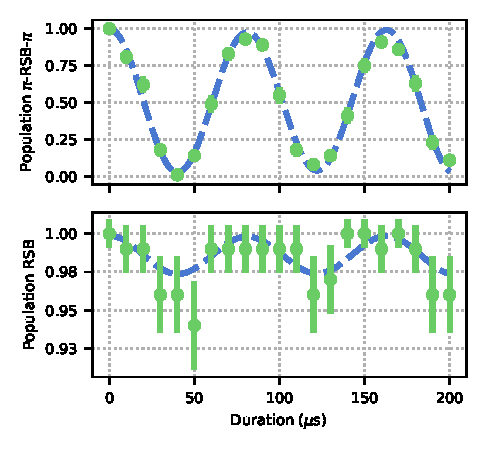
\includegraphics[width=\linewidth]{
            figures/pdf_figure/sideband_thermometry.pdf
            }
        \end{center}
        \caption{
            Thermometry after sideband cooling.
            }
        \label{fig:SBC}
    \end{figure}

    \begin{figure}
        \begin{center}
        \noindent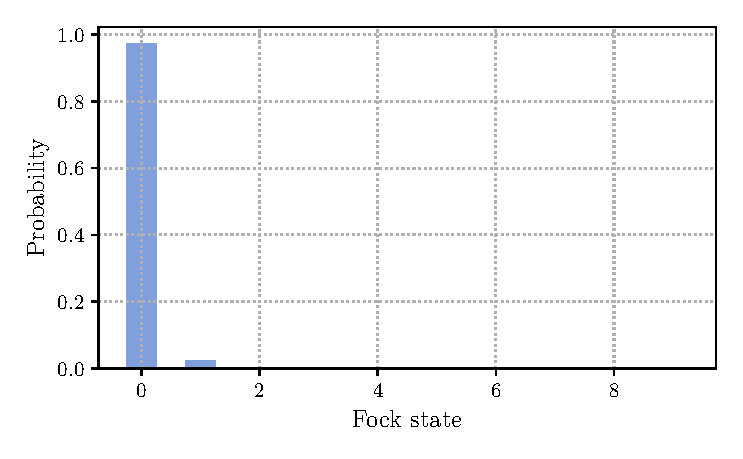
\includegraphics[width=\linewidth]{
            figures/pdf_figure/fock_state_distribution.pdf
            }
        \end{center}
        \caption{
            Fock state distribution
            }
        \label{fig:fock state}
    \end{figure}


    To further cool the ions toward their motional ground state, we use resolved
    sideband cooling. The motion of the ion, described by a harmonic oscillator,
    modulates the transition frequencies of the ion, leading to sidebands at
    multiples of the motional frequency. For the $4S_{1/2} \leftrightarrow
    3D_{5/2}$ transition, at appropriate laser intensity and motional mode
    frequencies, these sidebands can be resolved spectroscopically. The pulsed
    sideband technique we employ consists of red sideband pulses, followed by
    deshelving, and repumping pulses on the 854~nm and 866~nm transitions
    respectively. An example pulse sequence can be seen in
    figure~\ref{fig:sideband_cooling_sequence}, and experimental parameters we use are summarised in table~\ref{tab:cooling_parameters}.\\
    To verify the efficacy of our sideband cooling, we perform thermometry
    experiments by driving on resonance red sideband (RSB) and pi-RSB-pi pulse
    sequences. We record the time dynamics of population flopping as we vary RSB
    pulse length. In the case of Fock state zero, we expect to see a strong
    signal on the RSB, and no signal on the pi-RSB-pi pulses. We fit a thermal
    Fock state distribution (with truncation at Fock state = 100) to these
    signals to extract the mean occupation number, and $\eta\Omega$, the carrier
    Rabi frequency multiplied by the Lamb-Dicke parameter. A typical thermometry
    scan after Doppler and sideband cooling can be seen in
    figure~\ref{fig:sideband_cooling_results}. We find that the mean occupation
    number after sideband cooling is $\bar{n} = 0.03()$, and $\eta\Omega =
    XX$~MHz.\\
    Optimisation of the cooling parameters can be roughly performed by fitting
    temperature while scanning RSB pi-pulse durations, total number of pulses,
    repumping and deshelving times. One can optimise for minimum temperature,
    however it is also important to optimise for total cooling duration. For
    single ion, single mode experiments, this duration is often a non-issue,
    however for multi-ion crystals, any interaction involving the motion, may
    require the sequential sideband cooling of multiple motional modes. This can
    not be easily parallalised due to the requirement that the RSB pi-pulse is
    performed near resonance to one of the motional sidebands. This sequential
    cooling strategy can be either limiting when heating and cooling rates are
    comparable, or in the best case, painful due to long data collection times.\\
    To mitigate this issue, other sub-Doppler cooling techniques with larger
    accepted frequency bandwidths may be employed. Examples are dark-resonance
    cooling[], and electromagnetically induced transparency (EIT) cooling[], and
    Sisyphus cooling[]. These techniques are not yet implemented in our system,
    but will be likely additions once we move to larger ion crystals.\\

\subsection{Heating Rates}
\label{sec:Heating}
% Main points:
    % Quote motional heating rates for mode we use (have access to).
    % Describe heating model?
% Pre reqs:
    % Thermometry
    % Motional modes
    % Trap

    \begin{figure}
        \begin{center}
        \noindent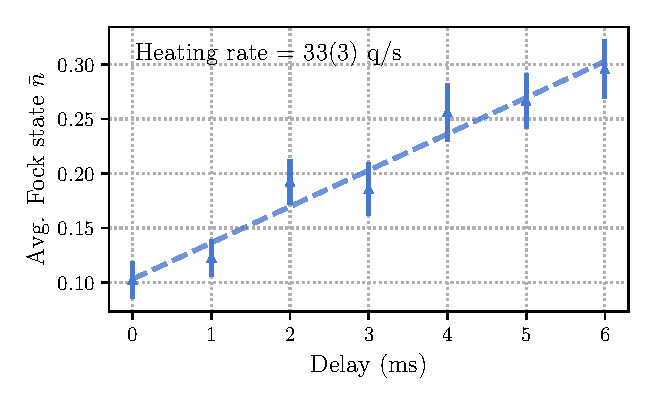
\includegraphics[width=\linewidth]{
            figures/pdf_figure/heating_rate.pdf
            }
        \end{center}
        \caption{
            Heating rates of upper radial mode.
            }
        \label{fig:heating rates}
    \end{figure}

    As mentioned, the cooling of our ions is only relevant if we have acceptable
    heating rates. Heating of the motion is predominantly caused by the ion trap
    itself. This can be due to imperfections in the surface of exposed
    dielectric and metals causing stray fields, or can be due to noise on the DC
    and RF drive voltages[]. Noise due to the surface of the trap can be
    mitigated by increasing ion-electrode distances, or by using traps with
    smaller surface area direclty exposed to the ion. In our case, as mentioned
    in sections~\ref{sec:The Ion Trap}, the NPL trap has an electrode ion
    distance somewhat larger than most surface traps, but less than that of a
    macroscope blade or rod style trap. To verify the heating rate of our
    system, we performed a series of thermometry scans whilst varying some delay
    time between cooling and thermometry pulses. A typical plot can be seen in
    figure~\ref{fig:heating_rate}. We find that the heating rate of our system
    is approximately $33(3)$~quanta per second on the upper radial 4~MHz mode on
    one ion.\\
    It is expected that the heating rate will be larger for lower frequency
    motional modes if we assume uniform electric field noise. We also verify
    this by looking at heating rate on the radial mode while varying the axial
    mode frequency. This is a useful diagnostic to check for unexpected heating
    at certain frequencies, perhaps due to RF noise in the lab. We find....\\

\subsection{Motional Mode Stability}
% Main points:
    % Quote motional mode drift 
    % Explain why it is currently drifty
    % Outline how this will be improved with the squareatron
% Pre reqs:
    % Trap

    \begin{figure}
        \begin{center}
        \noindent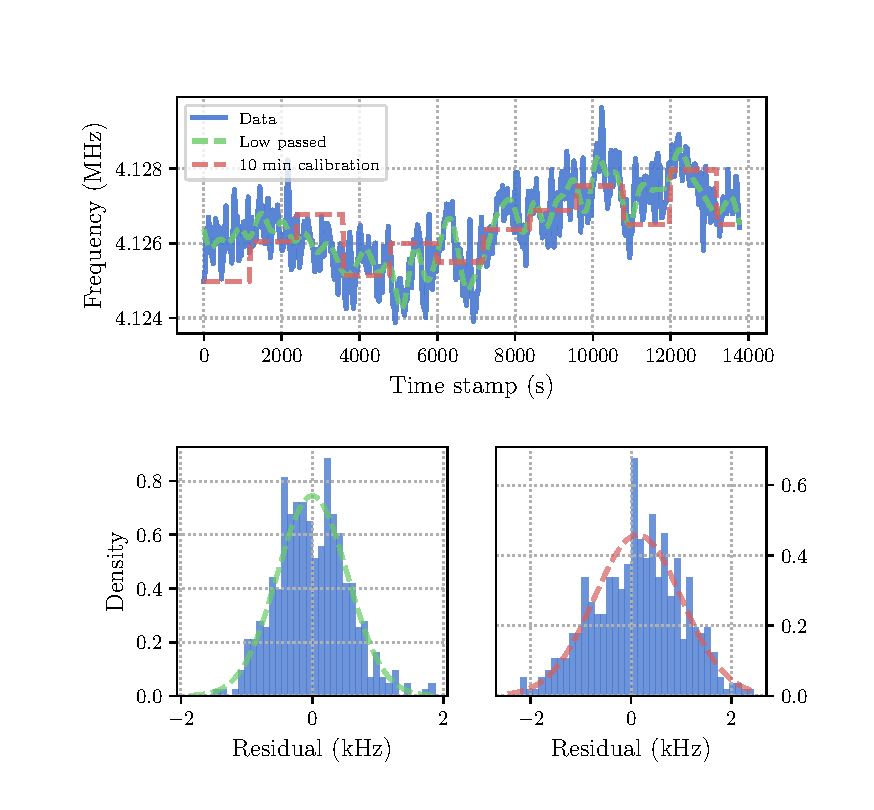
\includegraphics[width=\linewidth]{
            figures/pdf_figure/mode_drift.pdf
            }
        \end{center}
        \caption{
            Motional mode frequency drift.
            }
        \label{fig:mode drift}
    \end{figure}

\subsection{Motional Coherence Times}
% Main points:
    % Quote measured result for motional coherence time
    % Give estimate for what times we need for future experiments
    % Give estimate contributions from motional heating and from mode instability
    % What fix will we do for improving this - squareatron from prev section, resonator.
% Pre reqs:
    % Trap RF
    % Trap Resonator
    % Motional mode stability
    % SBC

\section{Spin-Dependent Forces}
\label{sec:Spin-Dependent Forces}
% Main points:
    % This is a primitive for motional control
    % This (we will see), is functionally a primitive for two qubit spin entanglement
    % Show equation as quite key to future work
% Pre reqs:
    % Motional mode spectra
    % 729 system
    % AOM control of 729

    \begin{figure}
        \begin{center}
        \noindent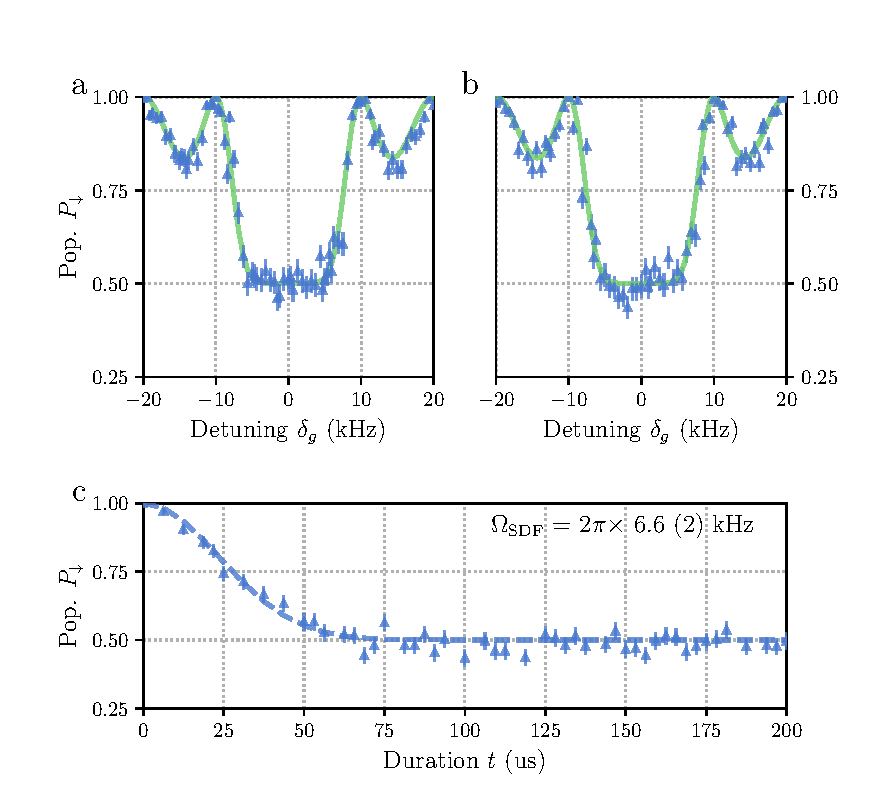
\includegraphics[width=\linewidth]{
            figures/pdf_figure/sdf.pdf
            }
        \end{center}
        \caption{
            SDF traces.
            }
        \label{fig:SDF}
    \end{figure}
    The spin-dependent force (SDF) is (planned to be) heavily used throughout
    this thesis. We use the Mølmer-Sørensen (MS) scheme~\cite{}, to generate the
    SDF via a bichromatic laser field. Bichromatic refers to the simultaneous
    application of two tones symmetrically detuned around the qubit carrier
    frequency, with absolute detuning approximately equal to the motional mode
    frequency, $\delta \approx \omega_{m}$. The resulting interaction, when
    ignoring off resonant and higher order couplings, is given by,
    \begin{equation}
        \hat{H}_{MS} = \hbar \eta\Omega~\hat{\sigma}_\phi\cos(\delta t) \left( a e^{-i\omega_{m} t} + a^\dagger e^{i\omega_{m} t} \right),
    \end{equation}
    where $\eta$ is the Lamb-Dicke parameter, $\Omega$ is the carrier Rabi
    frequency, $a(a^\dagger)$ is the lowering (raising) operator, and
    $\sigma_\phi$ is the Pauli operator with $\phi$ being in the $x,~y~$-plane.
    Applying the rotating wave approximation, and defining $\delta_g = \delta -
    \omega_{m}$, we find that the interaction Hamiltonian can be approximated
    to,
    \begin{equation}
        \hat{H}_{MS} = \frac{\hbar \eta\Omega}{2}~\hat{\sigma}_\phi \left( a e^{-i\delta_g t} + a^\dagger e^{i\delta_g t} \right).
    \end{equation}
    The SDF realises a displacement of the motional state in phase space. We may
    control the trajectory of this displacement by varying $\delta_g$: on
    resonance, $\delta_g = 0$, we see linear trajectories, whilst off resonance,
    $\delta_g \neq 0$, we see cyclic trajectories where after some time $t =
    2\pi/\delta_g$, the motion returns to the initial state. We shall exploit
    this control in both the two-qubit entangling gate experiments, as well as
    in the creation of squeezed states.\\

\subsection{Calibrating the SDF}
% Main points:
    % Here describe what error sources "look like"
    % Describe detuning and duration scans
    % Describe how we can detect these errors via the above strategy. Refer to OB thesis.
    % Fit an SDF with the errors?
% Pre reqs
    % Motional mode spectra
    % 729 system
    % AOM control of 729

    The MS interaction is widely used in ion trap experiments due to it being robust against varying intial motional states, and to the effects of heating during the pulse sequence. However, in our use case, the SDF is sensitive to miscalibration of the central qubit frequency, the balancing of power in the two tones, and to motional mode drifts. The first two miscalibrations appear as the SDF having..
    We use both ``detuning'' and ``duration'' scans to calibrate the SDF. The
    ``detuning'' scan is performed by varying the detuning, $delta_g$, of the interaction, whilst the keeping the SDF duration constant, whilst the ``duration'' scan keeps detuning constant and varies the SDF duration.
    Duration scan fit given by,
    \begin{equation}
        P_{\downarrow,\mathrm{th}} = \frac{1}{2} \left[ 1 + e^{-4\left( \bar{n} + \frac{1}{2} \right) |\alpha(t)|^2} \right],
    \end{equation}
    from Burd thesis, equation 3.30.
    $|\alpha(t)| = \Omega_{sdf} t/2$, fit find $\Omega_{SDF} = 2\pi\times 6.6(2)$~kHz, fitted with $\bar{n} = 0.03$
    Fitting detuning scan using
    $|\alpha(t)| = \Omega_{sdf} \sin(\delta t/2)/\delta$, find $\Omega_{SDF} = 2\pi\times 6.3(2)$~kHz, fitted with $\bar{n} = 0.03$.



\section{Two-Qubit Entangling Gates}
\label{sec:Two-Qubit Entangling Gates}
% Main points:
    % Intro/brief outline of goal of two-qubit gate. Truth table? Preparing in Bell state. This is tool kit for spin control of our system.
    % Discuss likely limitations being nearby hot motional modes, no pulse ramping
    % Current error vs what we expect we need for future experiments.
    % Here empasise that the SDF we discuss previously can be used to generate entanglement.
    % Showing phase coherence between operations is nice here.
% Prereqs:
    % SDFs
    % Single qubit gates
    % What available transitions we have
    % Motional mode spectra

    We perform two-qubit entangling gates using the Mølmer-Sørensen (MS)
    interaction~\cite{}. This interaction is the same described SDF from the
    previous section, but applied globally to two ions. The MS interaction
    relies on the spin dependent geometric phase accumulated during the motional
    displacement. To create a two-qubit entangled state, a differential
    geometric phase of $\pi/2$ must be accumulated between the two-qubit basis
    states. To ensure there is no residual motional entanglement, the final
    motional state must return to the initial state. In practise, using an SDF
    detuned by $\delta_g$, this is achieved by applying the MS interaction for a
    time $t = 2\pi/\delta_g$. The MS gate is a universal two-qubit gate, and
    along with only single qubit gates, constitutes a universal gate set for
    discrete quantum algorithms.\\  

    Here we quote the fidelity of experimentally demonstrated two-qubit gates on
    our system. The fidelity serves to quantify the ``closeness" or similarity of
    two density matrices.  For the use case of quantum information processing, what we
    care about is that the experimental unitary applied in the gate sequence closely resembles the unitary we desire theoretically. In general this
    means that we should measure the fidelity of the applied unitary in an input
    state agnostic way. Unfortunately this is often not practical as the input
    state space can be unwieldly, and the act of preparing the input state can
    also be error prone. As a compromise we can apply the test unitary to either
    one, or to a set of input states, and measure the fidelity of the output state
    with respect to the known target state. If the error mechansisms of the test
    unitary are well understood, arguments can be made that this measured
    fidelity for a set of input state is representative (or not representative)
    of the average fidelity over the input state space.\\
    Here for a two-qubit entangling gate, we target the creation of the Bell
    state $|\Phi^+\rangle = 1/\sqrt{2} \left( |00\rangle +
    e^{i\phi_0}|11\rangle \right)$, from an initial state of $|11\rangle$.
    The fidelity between our mixed state $\rho$, and the pure Bell state may be
    given by,
    \begin{equation}
        \mathcal{F} = \langle \Phi^+ | \rho | \Phi^+ \rangle = \frac{1}{2} \left( \rho_{00,00} + \rho_{11,11} \right) + \frac{1}{2}\left( e^{i\phi_0}\rho_{11,00}+e^{-i\phi_0}\rho_{00,11}\right),
        \label{eq:Fidelity}
    \end{equation}
    To extract the fidelity experimentally we follow the popular
    protocol~\cite{XXX}, where the first bracketted term of
    equation~\ref{eq:Fidelity} is measured by performing projective measurements
    of the two ions after the gate sequence to extract populations, and the second bracketted term,
    known as the coherence terms, are measured by applying a global analysis
    $\pi/2|_\phi$ pulse to the two ions and applying parity measurements. The
    contrast of the parity oscillations when varying the phase $\phi$ of the
    $\pi/2$ pulse yields the desired coherence term magnitude and phase. We require the creation of a Bell state for two qubit entangling, however do not care what basis this state is in, and so float the target Bell state phase and take only the magnitude of the fitted parity oscillations for calculating the final fidelity.\\

    The best two-qubit entangling gate fidelity currently achieved on our system is $\mathcal{F}=92(2)\%$. As shown in figure~\ref{fig:ms_gate}, the magnitude of the parity scan was measured to be 0.90(2), while the populations $\left( \rho_{00,00} + \rho_{11,11} \right) = 0.95(2)$. Each population point in these figures are found by taking the average of 200 shots of the gate sequence.\\

    These results serve as both a proof of principle for full spin control on
    our system, but also as a benchmark to which we can compare future system
    improvements.  For future work, we will require the use of this entangling
    gate either as Bell state preparation for input to analogue simulation
    experiments~\cite{}, or as a primitive gate for the spin component of hybrid
    algorithms~\cite{}.  In both these cases, especially any use that requires
    multiple concatenated entangling gates, we will likely require improved gate
    fidelities. It is suspected that we are currenlty limited by nearby hot
    motional modes, and the lack of pulse ramping in our gate sequence. We
    expect that with the addition of pulse shaping we will be able to suppress
    the effect of nearby off-resonant transitions, and by sideband cooling of
    nearby motional modes we will futher suppress contributions from unwanted
    spin-motion couplings.\\

    \begin{figure}
        \begin{center}
        \noindent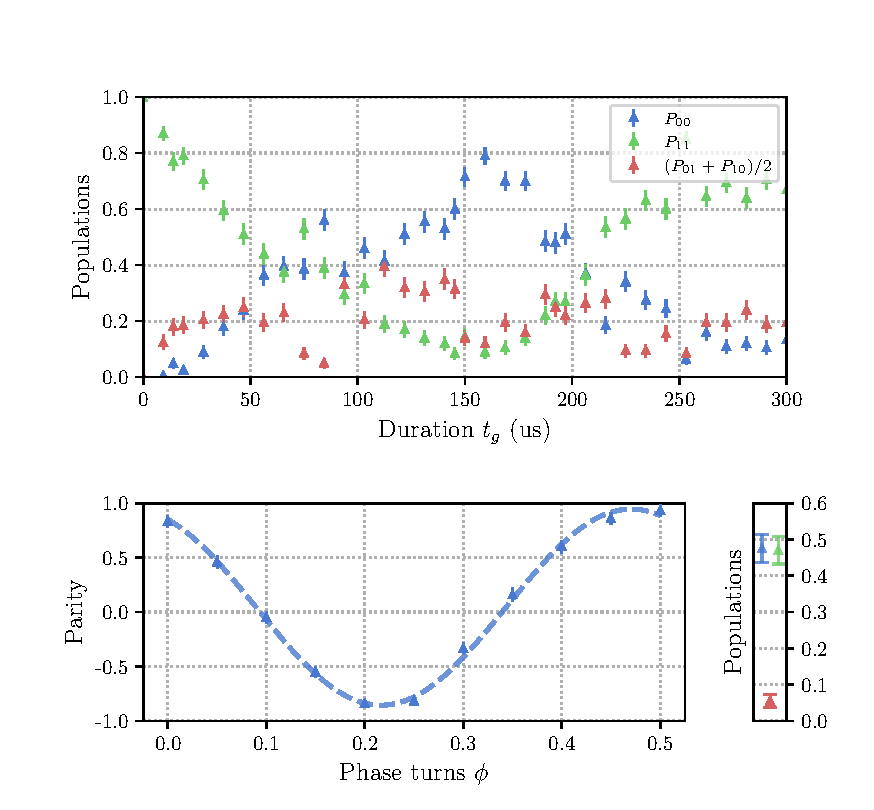
\includegraphics[width=\linewidth]{
            figures/pdf_figure/ms_gate.pdf
            }
        \end{center}
        \caption{
            MS Gate.
            }
        \label{fig:ms_gate}
    \end{figure}

\section{Creating Squeezed States}
\label{sec:Squeezed States}
% Main points:
    % Creating two simultaneous SDFs (requires section on SDFs!)
    % Four tones on one AOM
    % Phase relationships between SDFs (requires description of urukul?)
    % Limitations due to motional mode stability

% Prereqs:
    % SDFs
    % Motional characterisations

% ------------------------------------------------------------------------

\chapter{Outlook}

% Here I would like to briefly describe the next steps in the project, as well
% as the future experiments we want to demonstrate.
% Discussion of single addressing could be here.

% ------------------------------------------------------------------------

\clearpage


\clearpage
\section{Appendix}

\subsection{Generating Ions}
% Main points:
    % Atomic oven 
        % Really this is just for future members.
        % What temperature/current we go to
    % PI lasers
        % What powers/ saturation/ frequencies we use for trapping
        % Concerns of charging the trap with the UV lasers
% Pre reqs:
    % Atomic source

\subsection{Extracting Laser Offset and Magnetic Field}
\label{sec:Laser Offset}
% Main points:
    % How we fit out laser offset and field using multiple transitions
    % We have cavity and magnetic field drift.
    % We are on a magnetically sensitive transition
% Pre reqs:
    % The MUMetal box
    % 5 G field

\section{Experimental Control}
\label{sec:Experimental Control}
% figures for section
    % Recrystallisation routines
    % Autoload routines
    % Morningly calibrations

\end{document}